\section{Projeto de Banco de Dados}
\label{sec:titSecBancoDados}

Segundo \cite{silberschatz2006sistema}, o objetivo do projeto de Banco de Dados é a construção de um conjunto de estruturas que permitam a representação de um dado de forma não redundante e que esse dado possa ser recuperado de forma simples. Este processo geralmente passa em diferentes níveis de abstração. Primeiramente, inicia-se com o entendimento do problema, para depois seguir por diferentes fases de modelagem, até chegar à implementação. Nesse processo, um modelo considerado padrão para a etapa inicial de modelagem é o entidade-relacionamento (ER) \cite{heuser2009projeto}.

\subsection{Diagrama de Entidade-Relacionamento}
\label{sec:titSecDiagER}

A modelagem entidade-relacionamento é a mais utilizada e difundida técnica de modelagem de dados. Nesta técnica, o modelo de dados é representado por meio de um modelo entidade-relacionamento (modelo ER). Comumente, o modelo ER é representado graficamente por meio de um diagrama entidade-relacionamento (DER) \cite{heuser2009projeto}.

A \autoref{fig:diagramaer} representa o DER do projetado neste documento.

\begin{figure}[H]
    \centering
    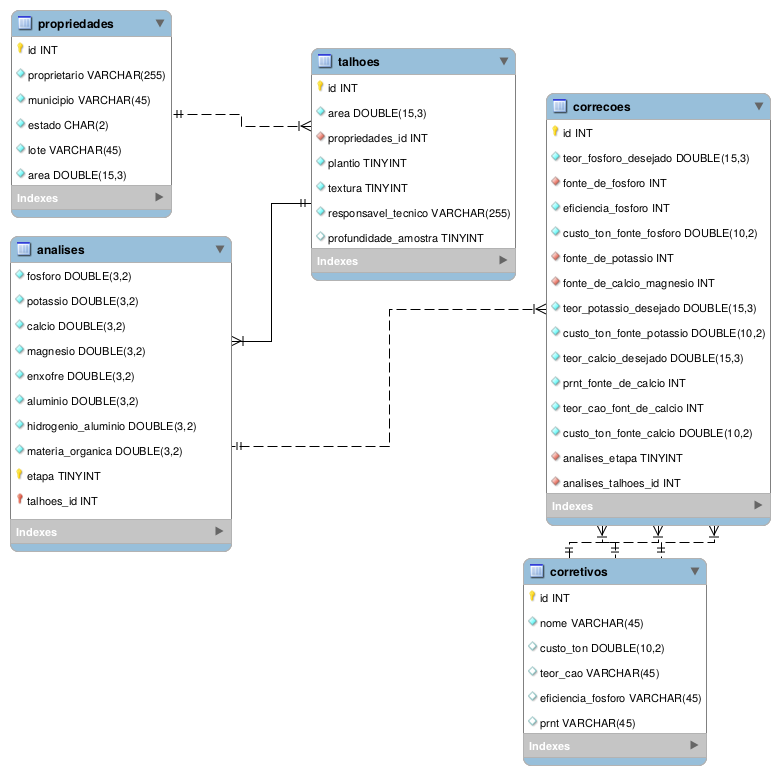
\includegraphics[width=13cm]{./dados/analise/diagramaer.png}
    \caption{Diagrama Entidade-Relacionamento}
    \label{fig:diagramaer}
\end{figure}

\subsection{Dicionário de Dados}
\label{sec:titSecDiagERDicionario}

\begin{landscape}
    \subsubsection{Tabela de Propriedades}
    \label{sec:titSubSecPropriedades}

    \begin{table}[H]
        \centering
        \caption[Tabela \textbf{propriedades}]{Na tabela propriedades ficarão armazenados os dados referentes à propriedade.
            \label{tab:tabela-er-propriedades}}
        \begin{tabular}{|p{4cm}|p{3cm}|p{2cm}|p{1cm}|p{2cm}|p{8cm}|}
            \hline
            Atributo     & Classe       & Domínio  & Bytes & Restrição & Descrição            \\\hline
            id           & Determinante & Numérico & 4     & PK, AI    &                      \\\hline
            proprietario & Simples      & Texto    & 255   & NN        & Nome do proprietário \\\hline
            municipio    & Simples      & Texto    & 255   & NN        & e.g. Dois Vizinhos   \\\hline
            estado       & Simples      & Texto    & 2     & NN        & e.g. PR              \\\hline
            lote         & Simples      & Texto    & 20    & NN        & e.g Q-103            \\\hline
            area         & Simples      & Numérico & 255   & NN        & Em metros quadrados  \\\hline
        \end{tabular}
    \end{table}

    \subsubsection{Tabela de Talhões}
    \label{sec:titSubSecTalhoes}

    \begin{table}[H]
        \centering
        \caption[Tabela \textbf{talhões}]{Na tabela talhões serão armazenados os dados referentes aos talhões da propriedade.
            \label{tab:tabela-er-talhoes}}
        \begin{tabular}{|p{4cm}|p{3cm}|p{2cm}|p{1cm}|p{2cm}|p{8cm}|}
            \hline
            Atributo              & Classe       & Domínio    & Bytes & Restrição & Descrição                        \\\hline
            id                    & Determinante & Numérico   & 4     & PK, AI    &                                  \\\hline
            area                  & Simples      & Numérico   & 10    & NN        & Em metros quadrados              \\\hline
            propriedades\_id      & Composto     & Numérico   & 255   & FK, NN    & Referência à tabela propriedades \\\hline
            plantio               & Simples      & Enumeravel & 1     & NN        & e.g. 1 (Plantio Direto)          \\\hline
            textura               & Simples      & Enumeravel & 1     & NN        & e.g. 2 (Textura Média)           \\\hline
            responsavel\_tecnico  & Simples      & Texto      & 255   & NN        & e.g. Pedro Cecere Filho          \\\hline
            profundidade\_amostra & Simples      & Numérico   & 255   &           & Em centímetros                   \\\hline
        \end{tabular}
    \end{table}

    \subsubsection{Tabela de Análises}
    \label{sec:titSubSecAnalises}

    \begin{table}[H]
        \centering
        \caption[Tabela \textbf{análises}]{Na tabela análises serão armazenados os dados do laudo técnico referente ao talhão.
            \label{tab:tabela-er-analises}}
        \begin{tabular}{|p{4cm}|p{3cm}|p{2cm}|p{1cm}|p{2cm}|p{8cm}|}
            \hline
            Atributo             & Classe       & Domínio  & Bytes & Restrição & Descrição                          \\\hline
            fosforo              & Simples      & Numérico & 4     & NN        & centimol de carga/decimetro cúbico \\\hline
            potassio             & Simples      & Numérico & 4     & NN        & centimol de carga/decimetro cúbico \\\hline
            calcio               & Simples      & Numérico & 4     & NN        & centimol de carga/decimetro cúbico \\\hline
            magnesio             & Simples      & Numérico & 4     & NN        & centimol de carga/decimetro cúbico \\\hline
            enxofre              & Simples      & Numérico & 4     & NN        & centimol de carga/decimetro cúbico \\\hline
            aluminio             & Simples      & Numérico & 4     & NN        & centimol de carga/decimetro cúbico \\\hline
            hidrogenio\_aluminio & Simples      & Numérico & 4     & NN        & centimol de carga/decimetro cúbico \\\hline
            materia\_organica    & Simples      & Numérico & 4     & NN        & centimol de carga/decimetro cúbico \\\hline
            etapa                & Determinante & Numérico & 4     & PK, AI    &                                    \\\hline
            talhoes\_id          & Composto     & Numérico & 4     & PK, FK    & Referência à tabela talhoes        \\\hline
        \end{tabular}
    \end{table}

    \subsubsection{Tabela de Correções}
    \label{sec:titSubSecAnalises}

    \begin{table}[H]
        \centering
        \caption[Tabela \textbf{Correções}]{Na tabela Correções serão armazenados os dados úteis para o cálculo do equilíbrio e correção do solo.
            \label{tab:tabela-er-correcoes}}
        \begin{tabular}{|p{4cm}|p{3cm}|p{2cm}|p{1cm}|p{2cm}|p{8cm}|}
            \hline
            Atributo                    & Classe       & Domínio  & Bytes & Restrição & Descrição                         \\\hline
            id                          & Determinante & Numérico & 4     & PK, AI    &                                   \\\hline
            teor\_fosforo\_desejado     & Simples      & Numérico & 1     & NN        & em percentual                     \\\hline
            fonte\_de\_fosforo          & Composto     & Numérico & 4     & NN        & em referência à tabela corretivos \\\hline
            eficiencia\_fosforo         & Simples      & Numérico & 1     & NN        & em percentual                     \\\hline
            custo\_ton\_fonte\_fosforo  & Simples      & Numérico & 8     & NN        & em R\$/tonelada                   \\\hline
            fonte\_de\_potassio         & Composto     & Numérico & 4     & NN        & em referência à tabela corretivos \\\hline
            fonte\_de\_calcio\_magnesio & Composto     & Numérico & 4     & NN        & em referência à tabela corretivos \\\hline
            teor\_potassio\_desejado    & Simples      & Numérico & 1     & NN        & em percentual                     \\\hline
            custo\_ton\_fonte\_potassio & Simples      & Numérico & 8     & NN        & em R\$/tonelada                   \\\hline
            teor\_calcio\_desejado      & Simples      & Numérico & 1     & NN        & em percentual                     \\\hline
            prnt\_fonte\_de\_calcio     & Simples      & Numérico & 1     & NN        & em percentual                     \\\hline
            teor\_cao\_font\_de\_calcio & Simples      & Numérico & 1     & NN        & em percentual                     \\\hline
            custo\_ton\_fonte\_calcio   & Simples      & Numérico & 8     & NN        & em R\$/tonelada                   \\\hline
            analises\_etapa             & Composto     & Numérico & 4     & FK        & Referência à tabela talhoes       \\\hline
            analises\_talhoes\_id       & Composto     & Numérico & 4     & FK        & Referência à tabela talhoes       \\\hline
        \end{tabular}
    \end{table}

    \subsubsection{Tabela de Correções}
    \label{sec:titSubSecAnalises}

    \begin{table}[H]
        \centering
        \caption[Tabela \textbf{Corretivos}]{Na tabela Corretivos serão armazenados os dados padrões acerca dos corretivos.
            \label{tab:tabela-er-correcoes}}
        \begin{tabular}{|p{4cm}|p{3cm}|p{2cm}|p{1cm}|p{2cm}|p{8cm}|}
            \hline
            Atributo            & Classe       & Domínio  & Bytes & Restrição & Descrição       \\\hline
            id                  & Determinante & Numérico & 4     & PK, AI    &                 \\\hline
            nome                & Simples      & Texto    & 255   & NN        & em percentual   \\\hline
            custo\_ton          & Simples      & Numérico & 8     &           & em R\$/tonelada \\\hline
            teor\_cao           & Simples      & Numérico & 1     &           & em percentual   \\\hline
            eficiencia\_fosforo & Simples      & Numérico & 1     &           & em percentual   \\\hline
            prnt                & Simples      & Numérico & 1     &           & em percentual   \\\hline
        \end{tabular}
    \end{table}

\end{landscape}